\documentclass[12pt]{article}

\newcommand{\E}[1]{{\mathbf{E}[#1]}}
\newcommand{\Prob}[1]{{\mathbf{Pr}[#1]}}
\newcommand{\ProbSub}[2]{{\mathbf{Pr}_{#1}[#2]}}
\newcommand{\Var}[1]{{\mathbf{Var}[#1]}}
\newcommand{\Cov}[1]{{\mathbf{Cov}[#1]}}

\usepackage[authoryear,round]{natbib}
\usepackage{amsmath}
\usepackage{graphicx}
\usepackage{comment}
\usepackage{url}

\usepackage{subfigure}

\begin{document}

\date{}
\title{Modeling Distant Supervision and Heuristically Generated Training Data with Latent Variables}
\author{Alan Ritter}
\maketitle

\bibliographystyle{plainnat}

\section{Learning from Heuristically Labeled Training Data}
Many learning tasks require a large volume of annotated data; manual annotation of which is often costly or infeasible in practice.
In many scenarios there exists some external source of information which is very informative in predicting the target concept, but
can only be exploited in special circumstances (e.g. for specific entities in a database, or retrospectively in time).
To exploit these ``weak'' supervision signals, there has been a long history of research on heuristics for automatically annotating training data
for a wide variety of different tasks \citep{Agichtein01,Carlson10,Weld09,mintz09}.
A high level graphical model representation of this process of heuristically labeling training data for learning is presented in figure \ref{heuristic}.

\begin{figure}
  \centering
  \subfigure[Training]{
    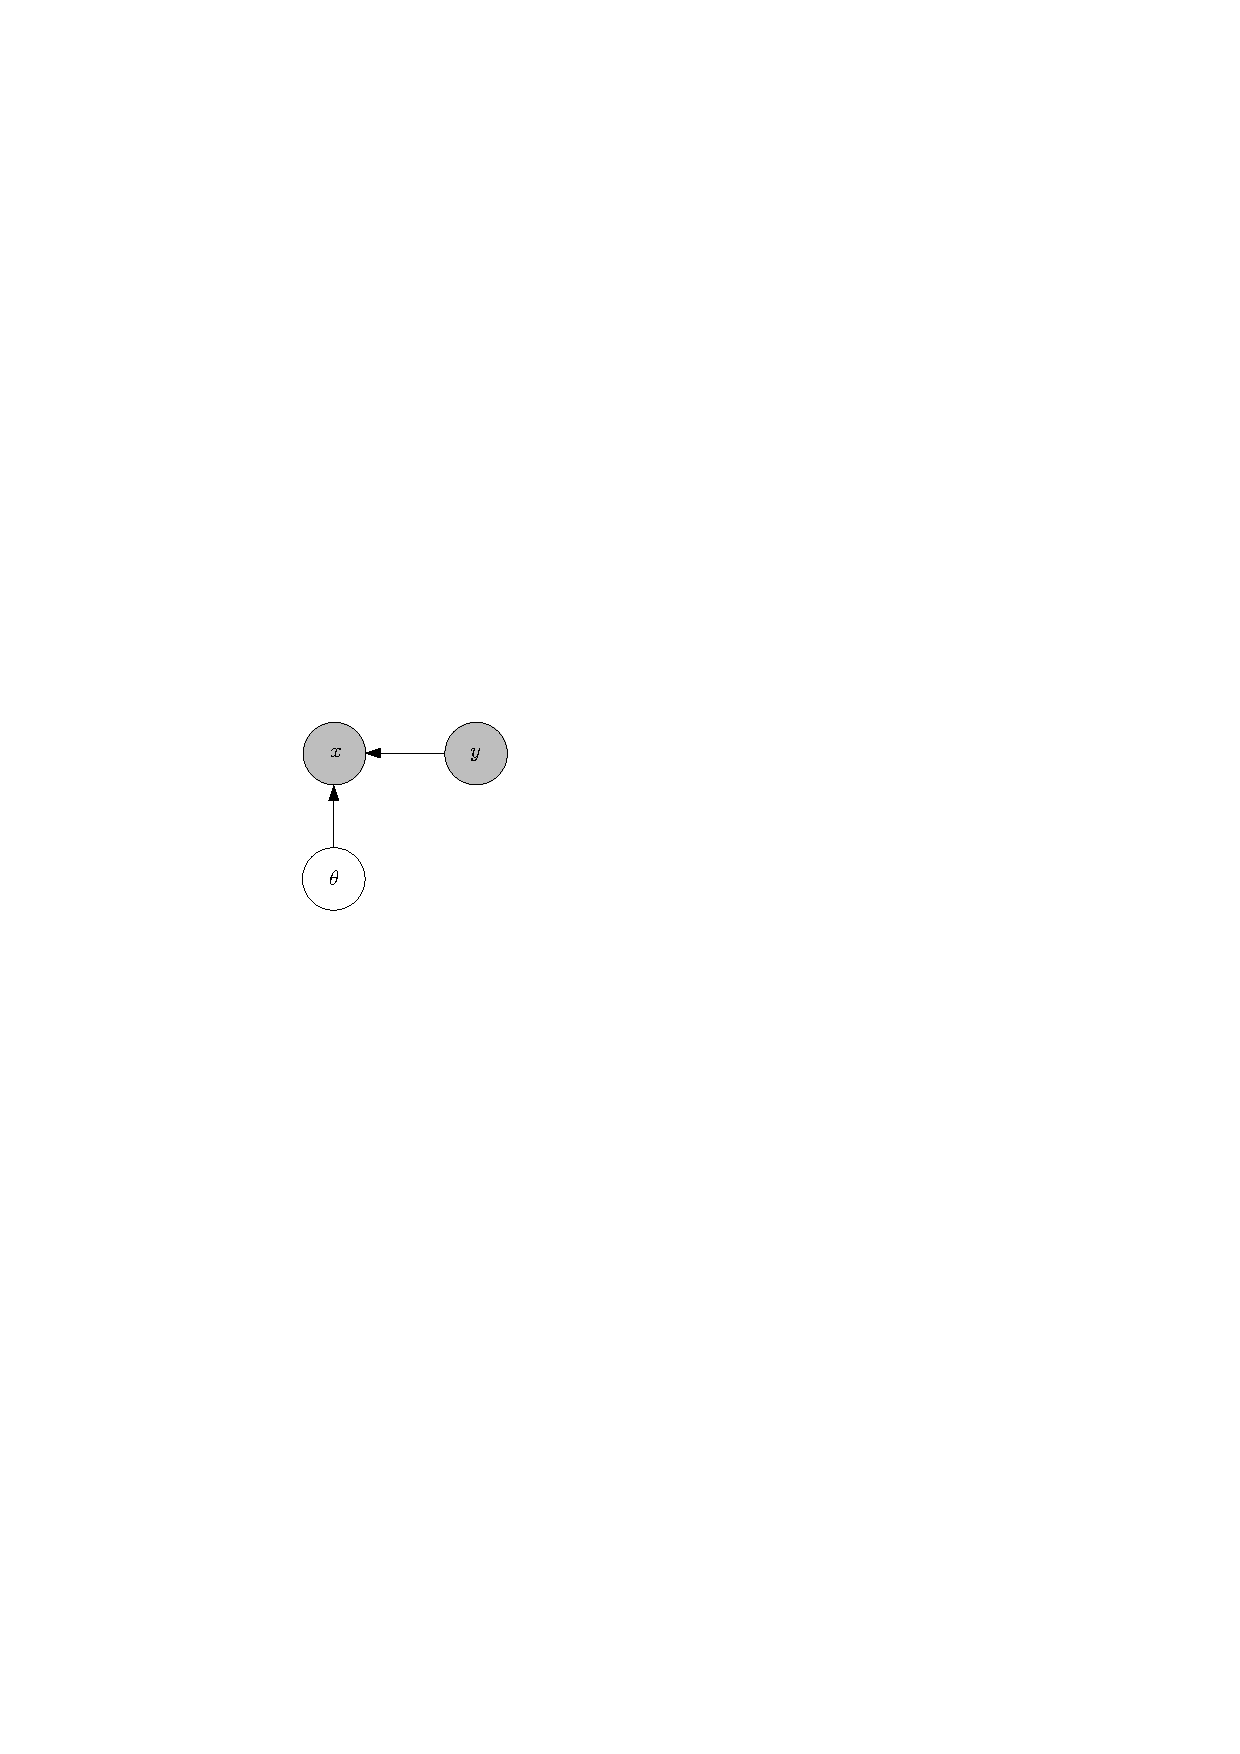
\includegraphics{supervised_train.pdf}
  }
  \subfigure[Testing]{
    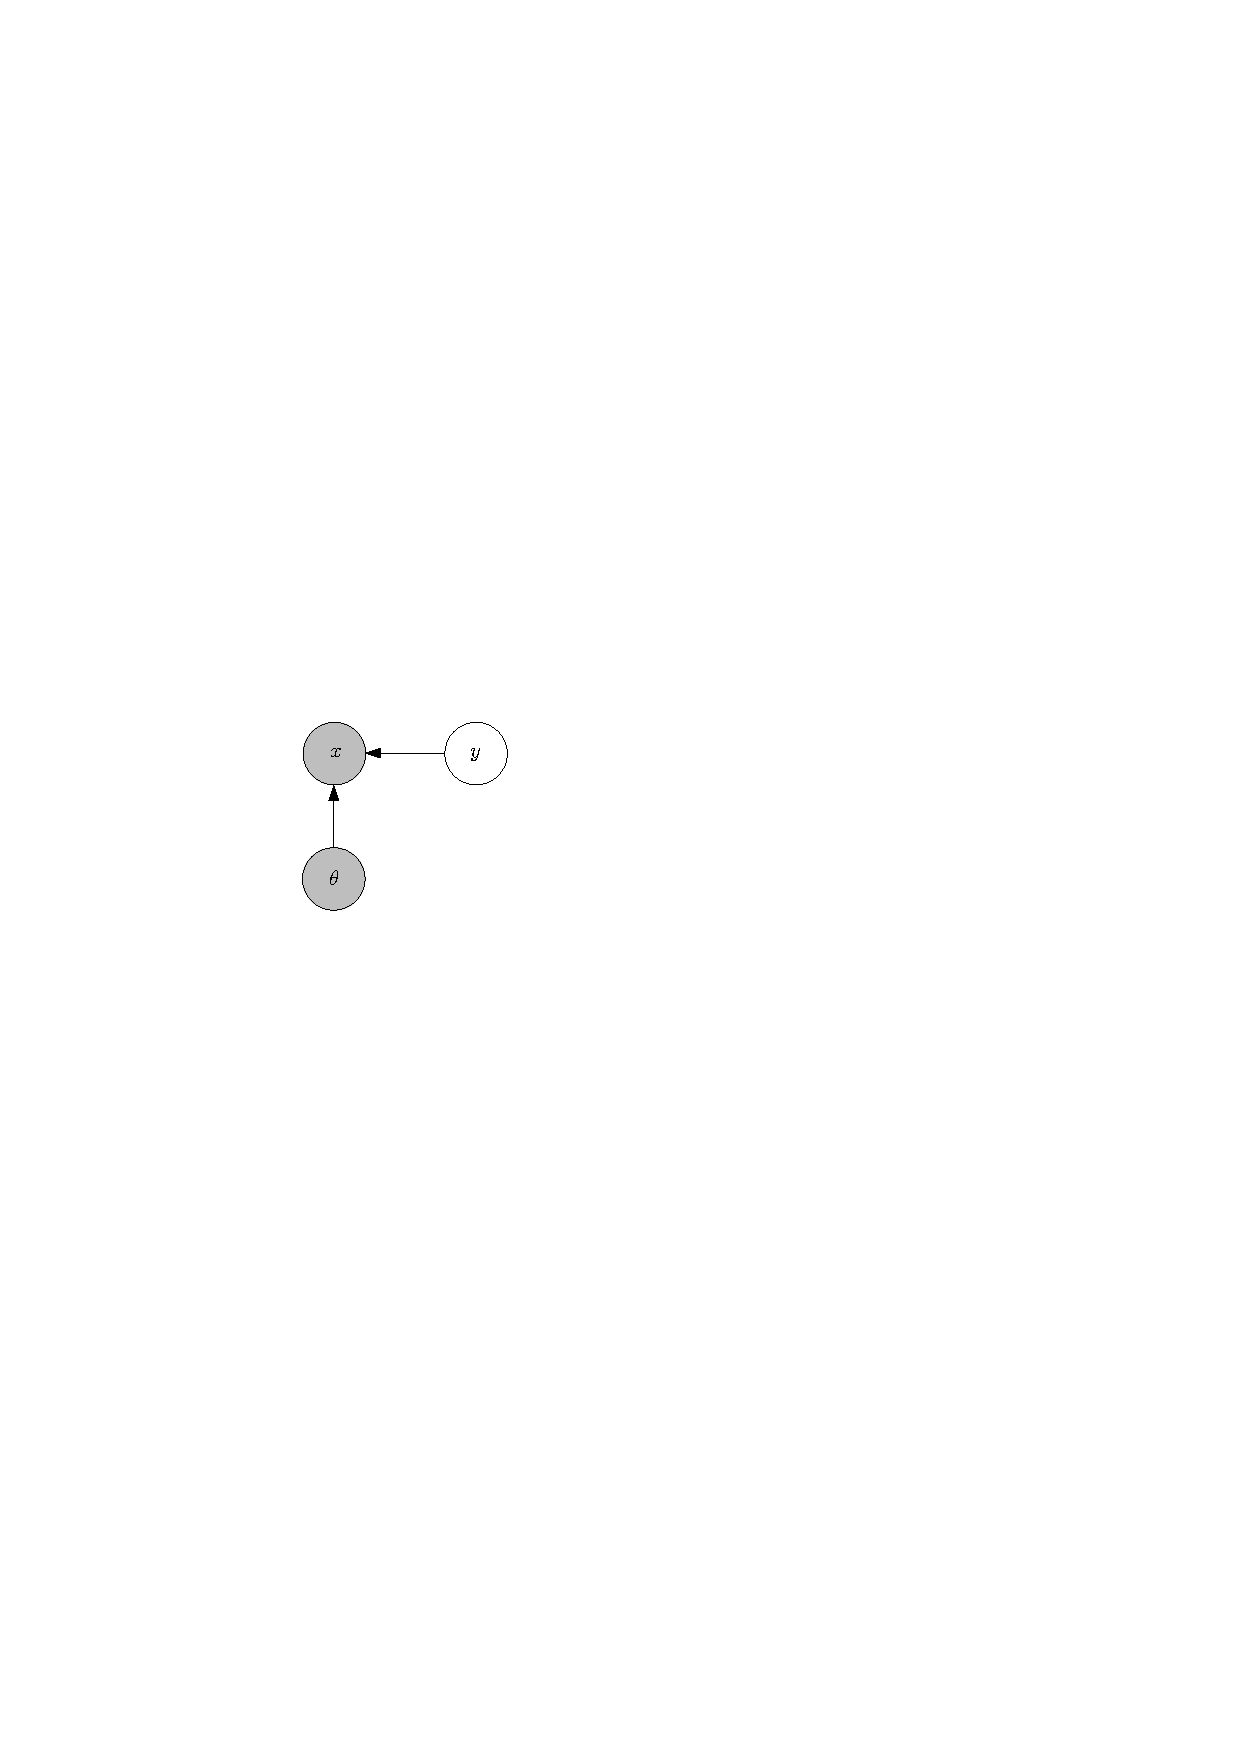
\includegraphics{supervised_test.pdf}
  }
  \caption{{\bf Supervised Learning}.  First parameters $\theta$ are learned when $x$ and $y$ are both observed.  Learned
  parameters are then used to infer $P(y|x)$ during testing.}
\end{figure}

In most cases there is a certain amount of ambiguity inherent in the labeling process.  For example a sentence mentioning ``Amazon''
may refer to either the {\sl COMPANY}, or the {\sl LOCATION}.  Most current approaches would deterministically label such
sentences with one label or the other, leading to noisy training data.
A better approach is to preserve the ambiguity inherent in training data automatically generated in this way, as illustrated
in Figure \ref{dlvm_train}.

\section{Relationship to Multiple Instance Learning}
Another established learning setup for modeling noisy / heuristically generated training data which was originally developed for 
a problem in drug design is \emph{Multiple Instance Learning}.  Clearly MIL is strongly related to the approach presented in Figure
\ref{dlvm_train}, however I believe it's assumptions are
not appropriate for modeling heuristically generated data in every situation.

\subsection{Example}
To demonstrate that at least MIL, and \emph{Multi-Labeled Learning} make different assumptions about the data, consider the following simple example:
\begin{description}
  \item[\bf Dictionaries]:
    \begin{itemize}
      \item {\sc Company}: \{Apple, Amazon, Microsoft, etc...\}
      \item {\sc Location}: \{Amazon, Sahara, Mexico, Seattle, etc...\}
      \item {\sc Food}: \{Apple, Banana, Taco, Burrito, etc...\}
    \end{itemize}
  \item[\bf Sentences]:
    \begin{itemize}
      \item {\bf Apple} acquired Siri.
      \item {\bf Amazon} acquired Kiva.
    \end{itemize}
\end{description}

\subsubsection{Representation using Multiple Instance Learning}
Using MIL, we might represent this noisily labeled training data using the following \emph{positive bags}
\begin{itemize}
  \item \{({\bf Apple} acquired Siri., {\sc Company})\}
  \item \{({\bf Apple} acquired Siri., {\sc Food})\}
  \item \{({\bf Amazon} acquired Siri., {\sc Company})\}
  \item \{({\bf Apple} acquired Siri., {\sc Location})\}
\end{itemize}
Note that two out of the 4 bags contain no positive examples, thus violating the assumptions made by MIL.

Alternatively, we could re-arrange the data into bags as follows:
\begin{itemize}
  \item \{({\bf Apple} acquired Siri., {\sc Company}),
    ({\bf Apple} acquired Siri., {\sc Food})\}
  \item \{({\bf Amazon} acquired Siri., {\sc Company}),
    ({\bf Apple} acquired Siri., {\sc Location})\}
\end{itemize}
Now it is true that each bag contains at least one positive instance, but note that MIL assumes each positive
bag contains \emph{one or more positive example}, when in fact a more appropriate assumption
in this circumstance is that each positive bag contains \emph{exactly one} positive example.

\begin{figure}
  \centering
  \subfigure[Labeling]{
    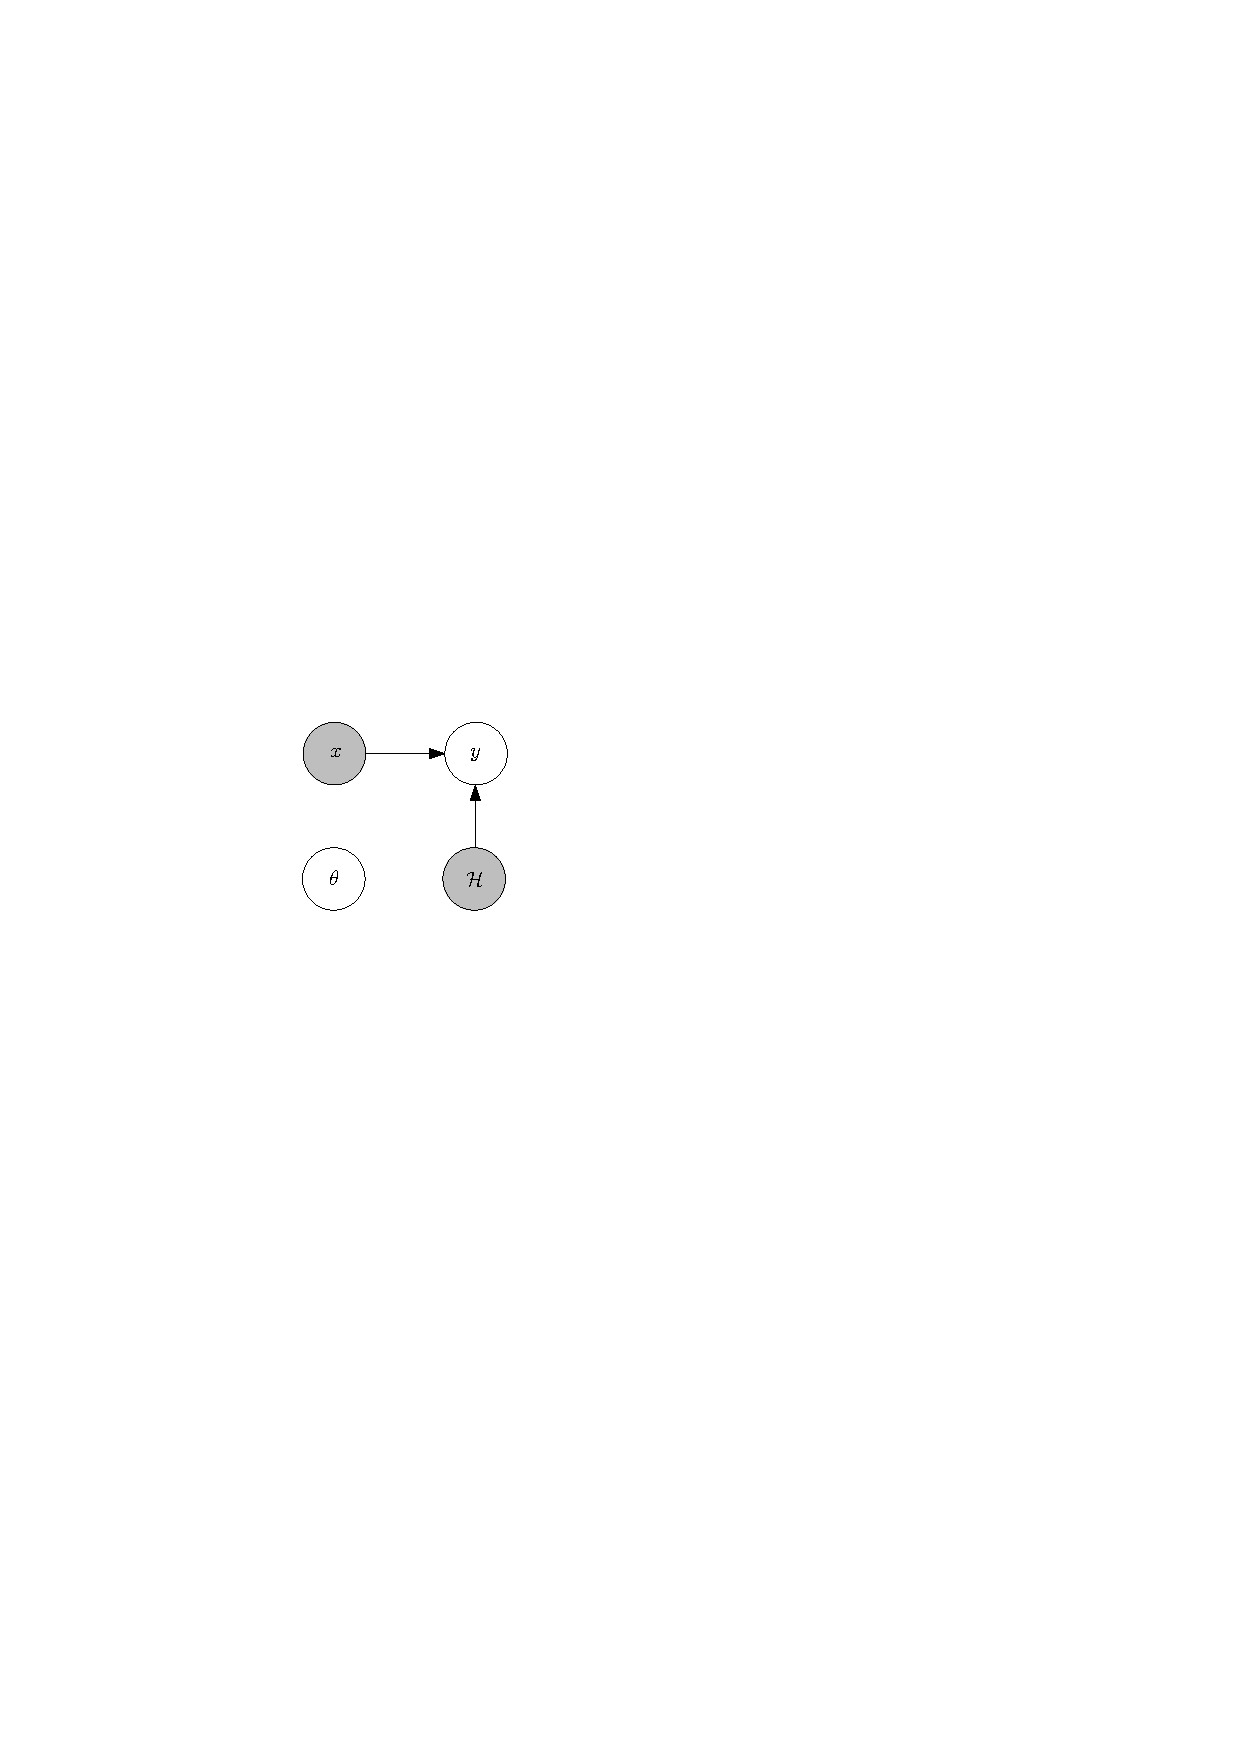
\includegraphics{heuristic_label.pdf}
  }
  \subfigure[Training]{
    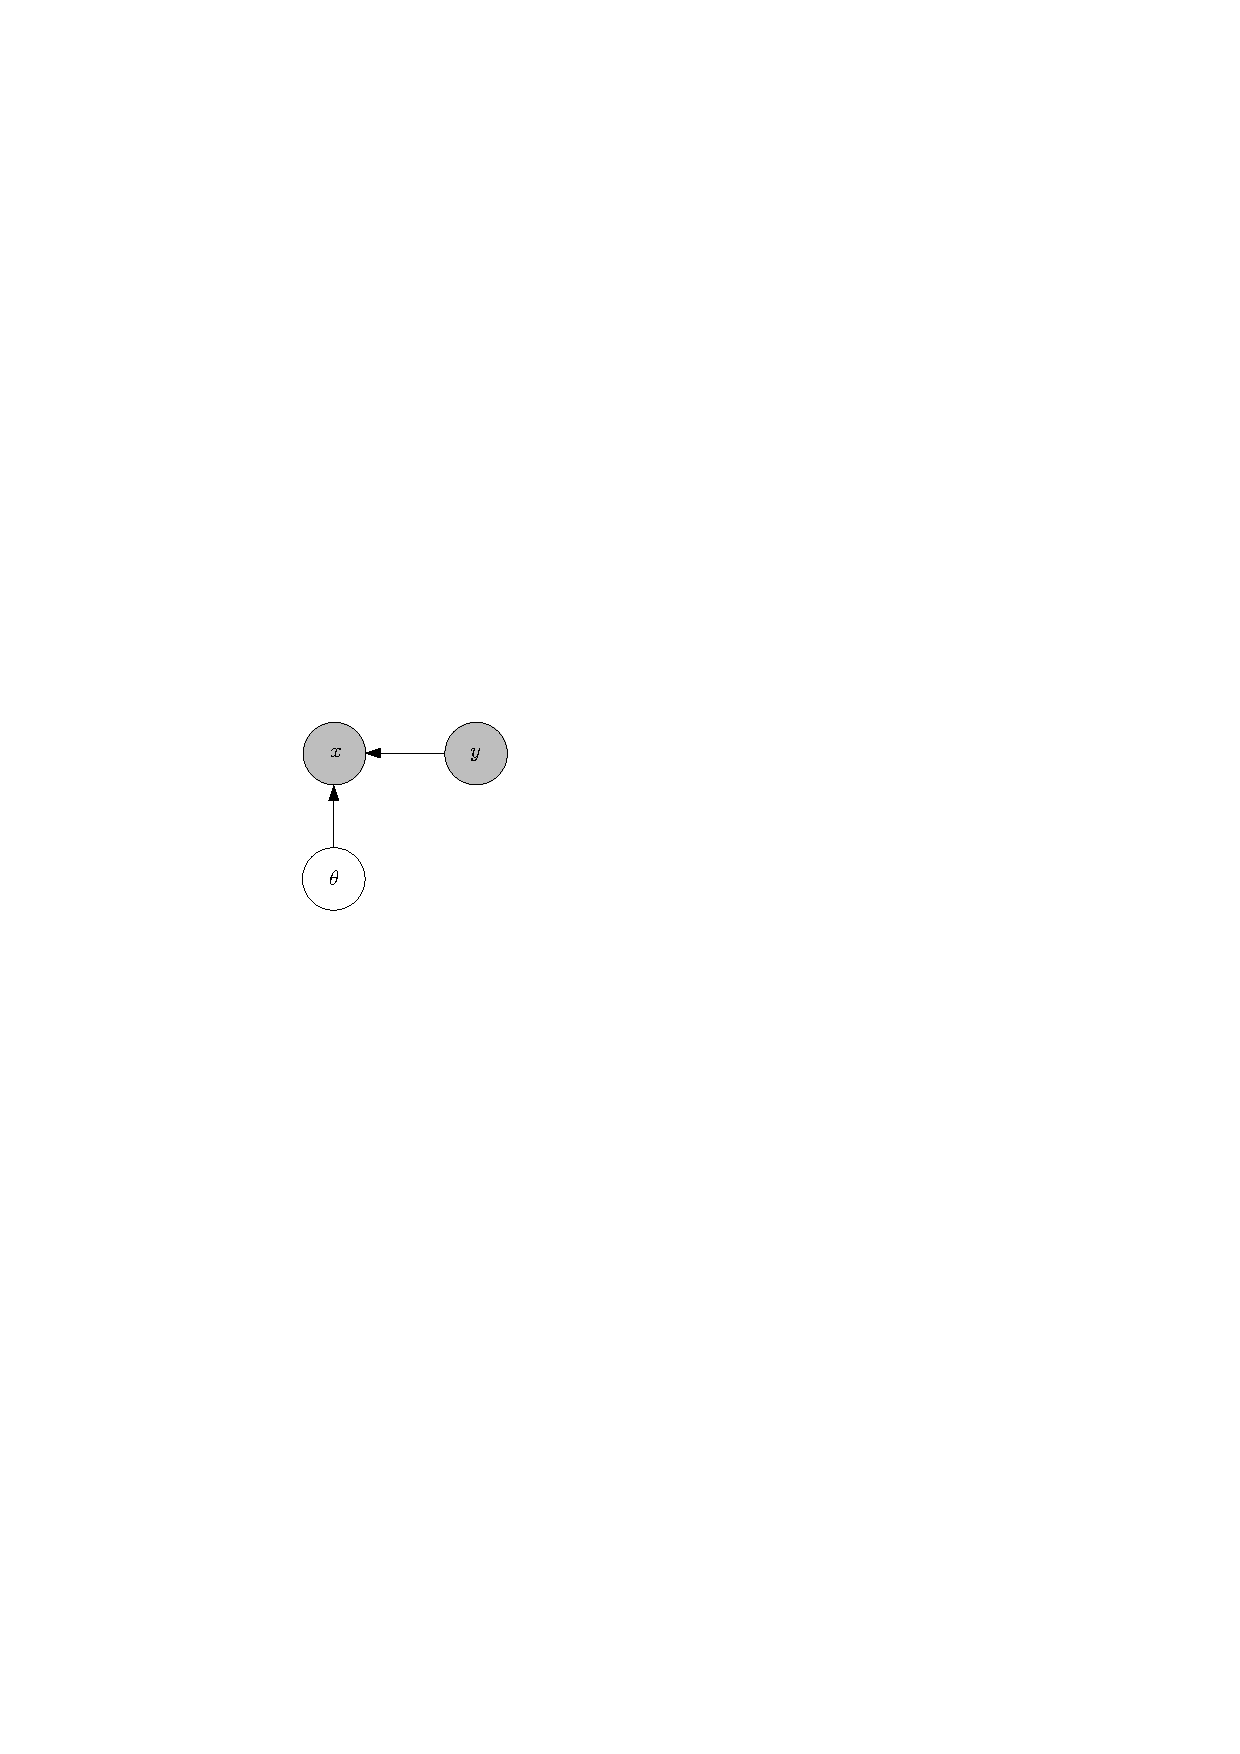
\includegraphics{heuristic_train.pdf}
  }
  \subfigure[Testing]{
    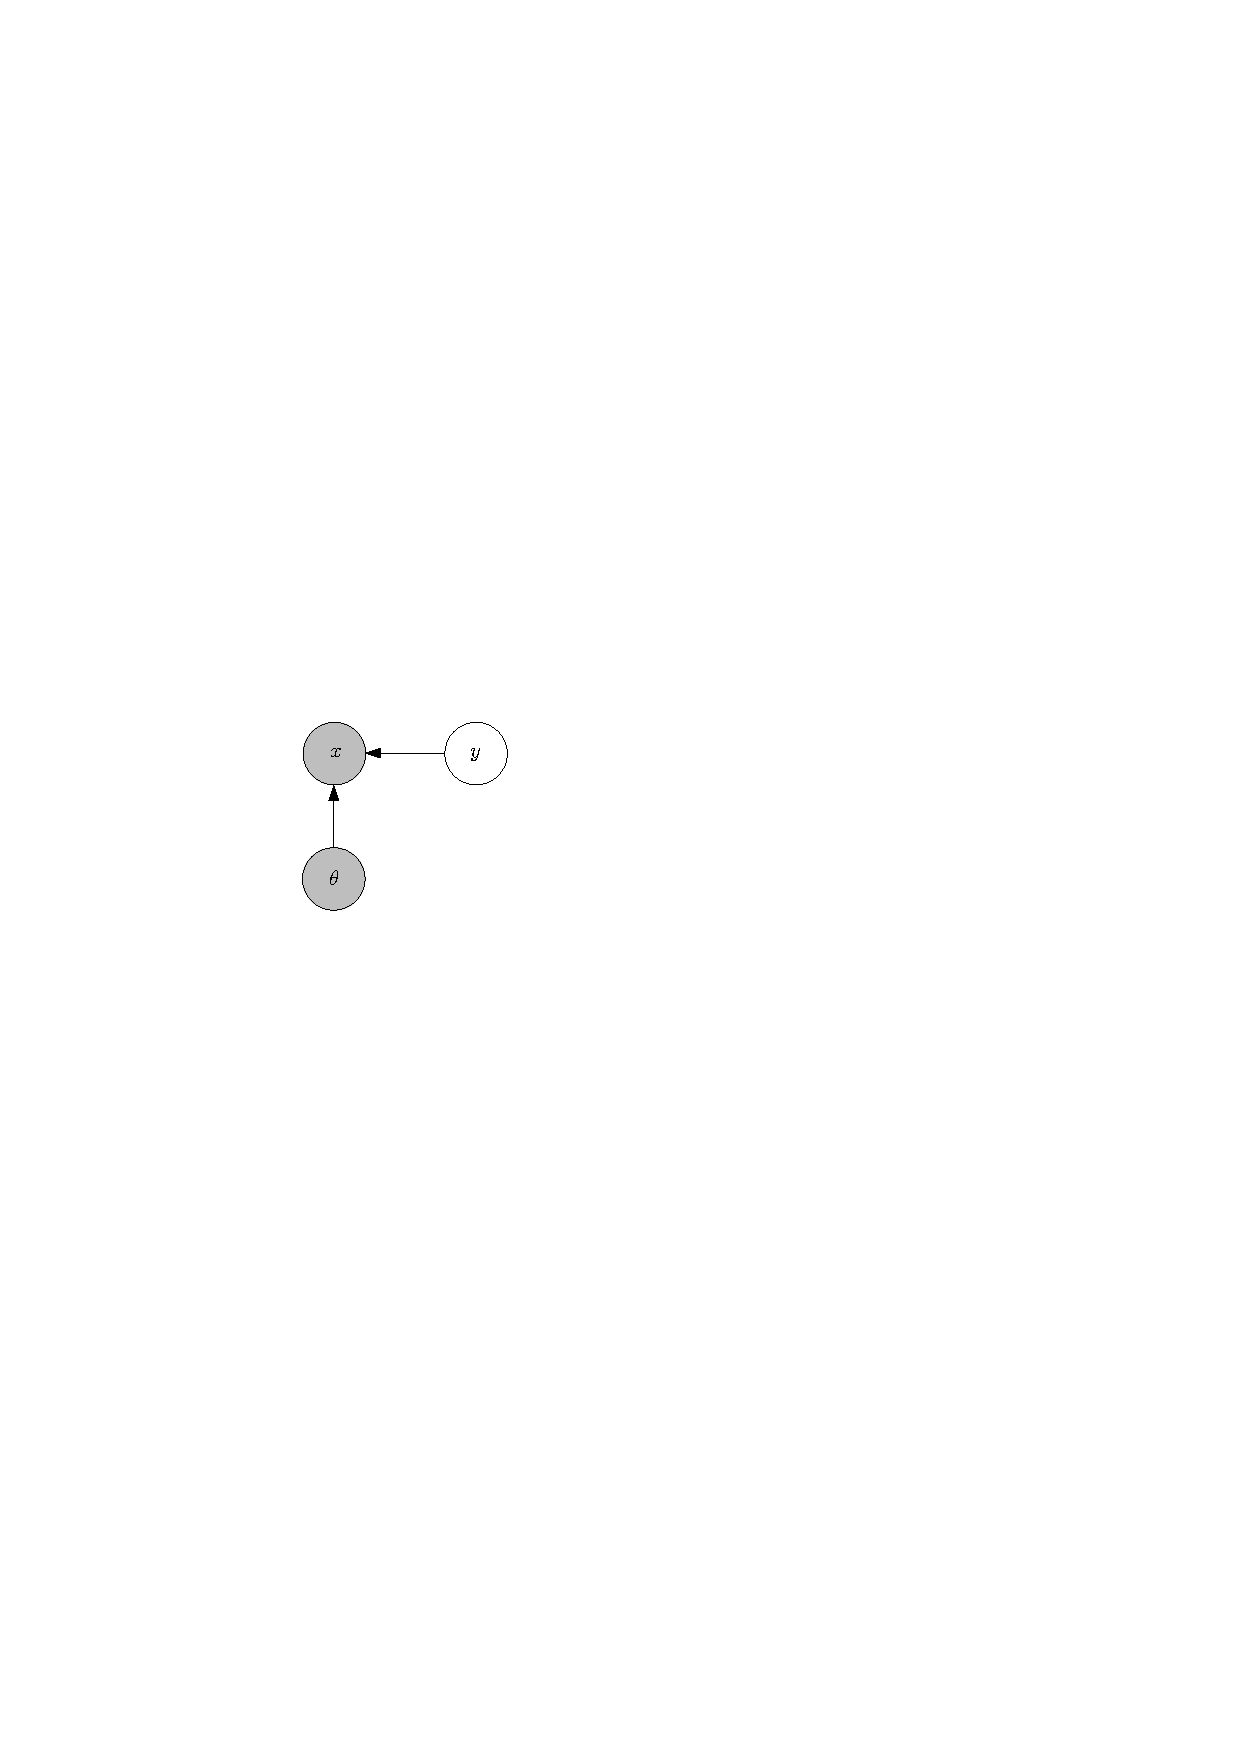
\includegraphics{heuristic_test.pdf}
  }
  \caption{{\bf Learning With Heuristically Labeled Training Data}.  $y$ is first labeled based on $x$ and a set of heuristics, $\mathcal{H}$.  Training
  and testing then proceed in the same way as supervised learning.}
  \label{heuristic}
\end{figure}

\begin{figure}
  \centering
  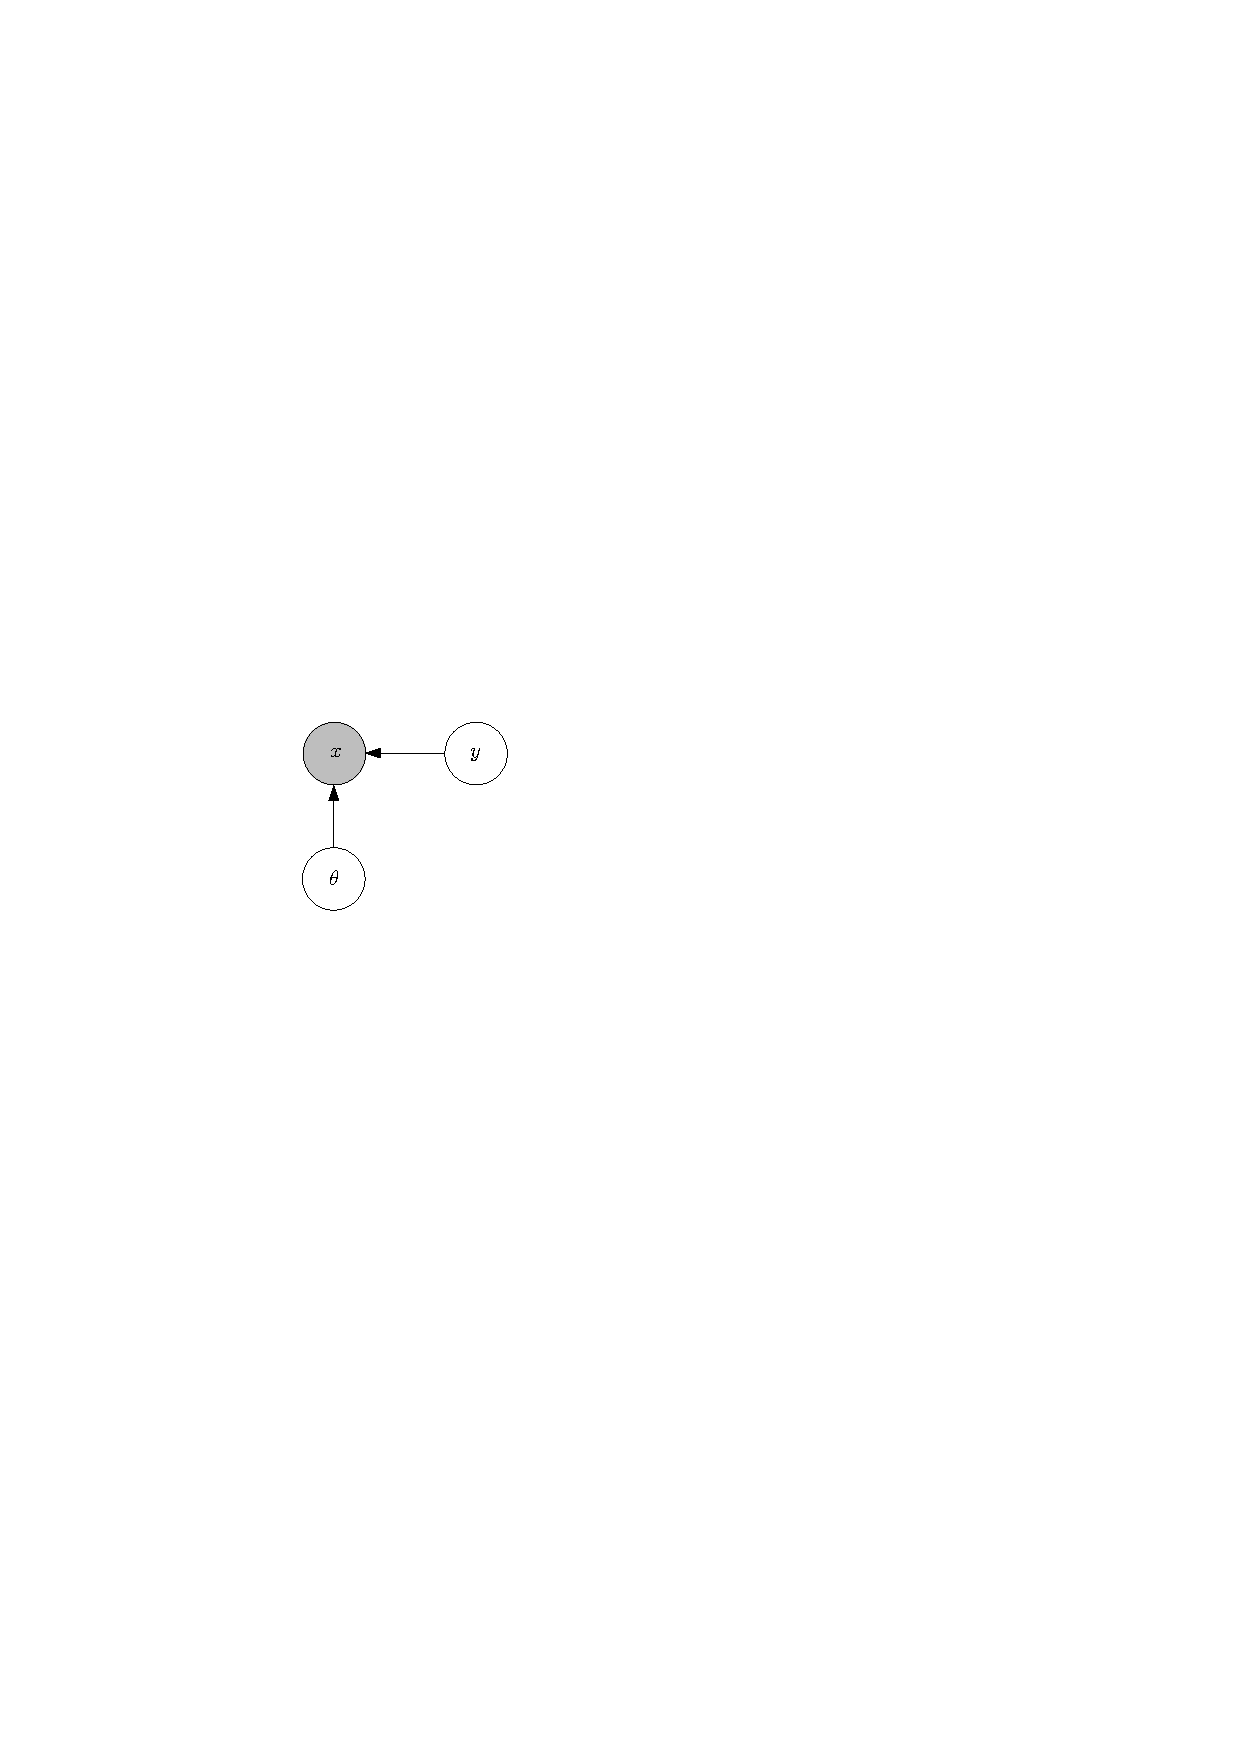
\includegraphics{unsupervised_train.pdf}
  \caption{{\bf Unsupervised Learning}.  Neither $y$ nor $\theta$ are ever observed.  Both are inferred based on $x$.}
\end{figure}

\begin{figure}
  \centering
  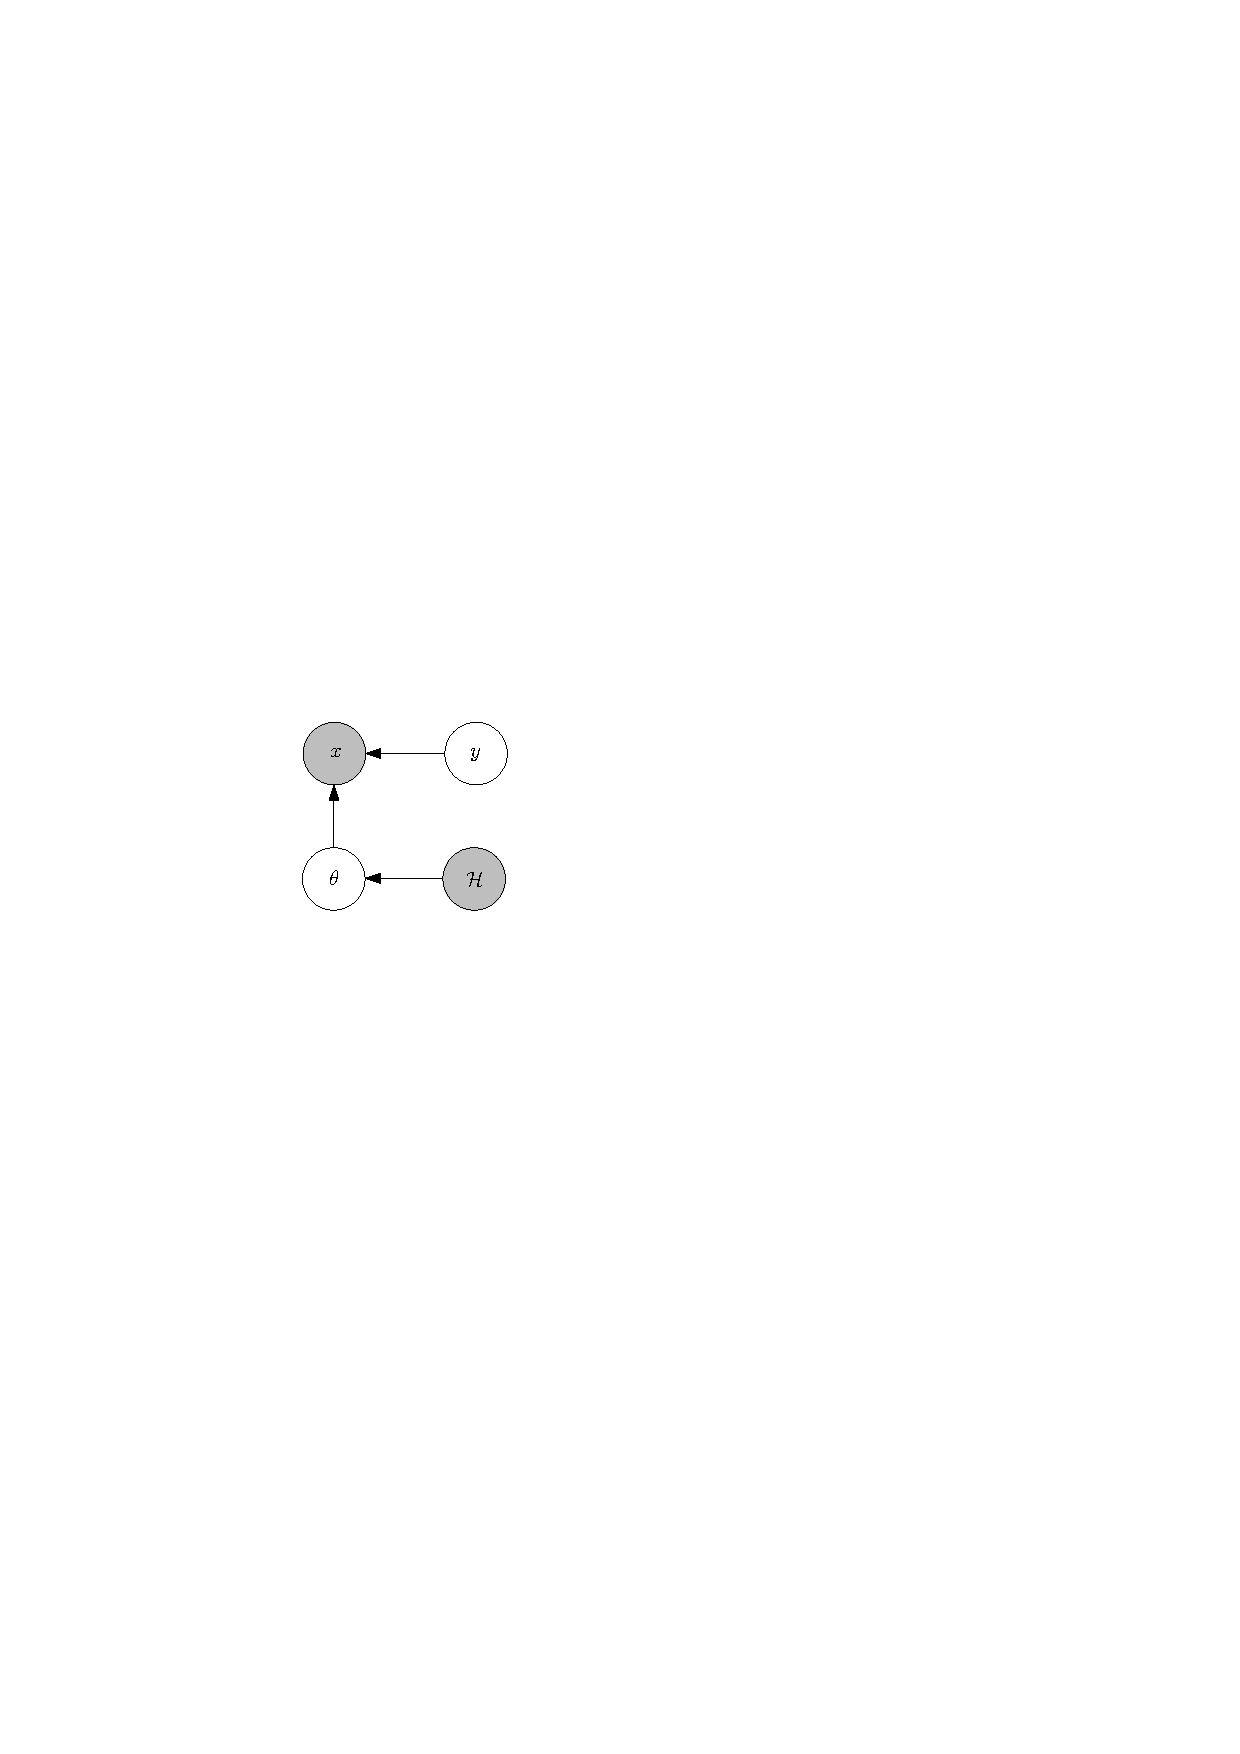
\includegraphics{dlvm_train.pdf}
  \caption{{\bf Learning with Heuristics as Constraints}.  Like the unsupervised case, both $y$ and $\theta$ are hidden (never observed),
  but heuristics are used to constrain the hypothesis space, (possible values of $\theta$).}
  \label{dlvm_train}
\end{figure}


\section{Applications}
The following sections describe several instances of this approach to specific applications.


\subsection{Entity Categorization}
\begin{description}
\item[Input:] Entity Mentions + Freebase Dictionaries
\item[Latent Variables:] Model the type of each entity
\item[Graphical model:] Latent Dirichlet Allocation (parameters constrained by Freebase Dictionaries)
\item[Empirical Results:] Outperforms Supervised Baseline (~2000 annotated tweets) and Co-Training.
\end{description}

\subsection{Relation Extraction}
\begin{description}
\item[Input:] Entity Pair Mentions + Freebase Relations
\item[Latent Variables:] Model the relation mentioned between each pair of entities
\item[Graphical Model:] Latent Dirichlet Allocation (parameters constrained by Freebase Relations)
\item[Empirical Results:] None
\end{description}

\subsection{Temporal Reference Resolution}
\begin{description}
\item[Input:] Sentences + Significant Events
\item[Latent Variables:] Model whether each word is part of a temporal expression and if so, what date property it refers to (e.g. MONTH=May, DOM=24, DOW=Thursday, etc...)
\item[Graphical Model:] Hidden Markov Model (parameters constrained by properties of the date associated with the mentioned event).
\item[Empirical Results:] None
\end{description}

\section{Relaxing the Closed World Assumption}
One assumption we have been making so far is that for each instance, at least one label generated according to the heuristics $\mathcal{H}$ is correct.
To relax this assumption one option would be a generative model of facts stated in the database (or heuristics) and the text, as illustrated in
Figure \ref{generative}.

The truth ($\mathcal{T}$) of each possible ground fact $f$ could be modeled with a latent variable.  The probability of each fact being observed
as part of the heuristic labels $\mathcal{H}$ would depend on whether the fact is true or false:

$$
P(d|f) = \left\{ \begin{array}{rl}
 0.5 &\mbox{ if $f=\text{true}$} \\
 0   &\mbox{ if $f=\text{false}$}
       \end{array} \right.
$$

\begin{figure}
  \centering
  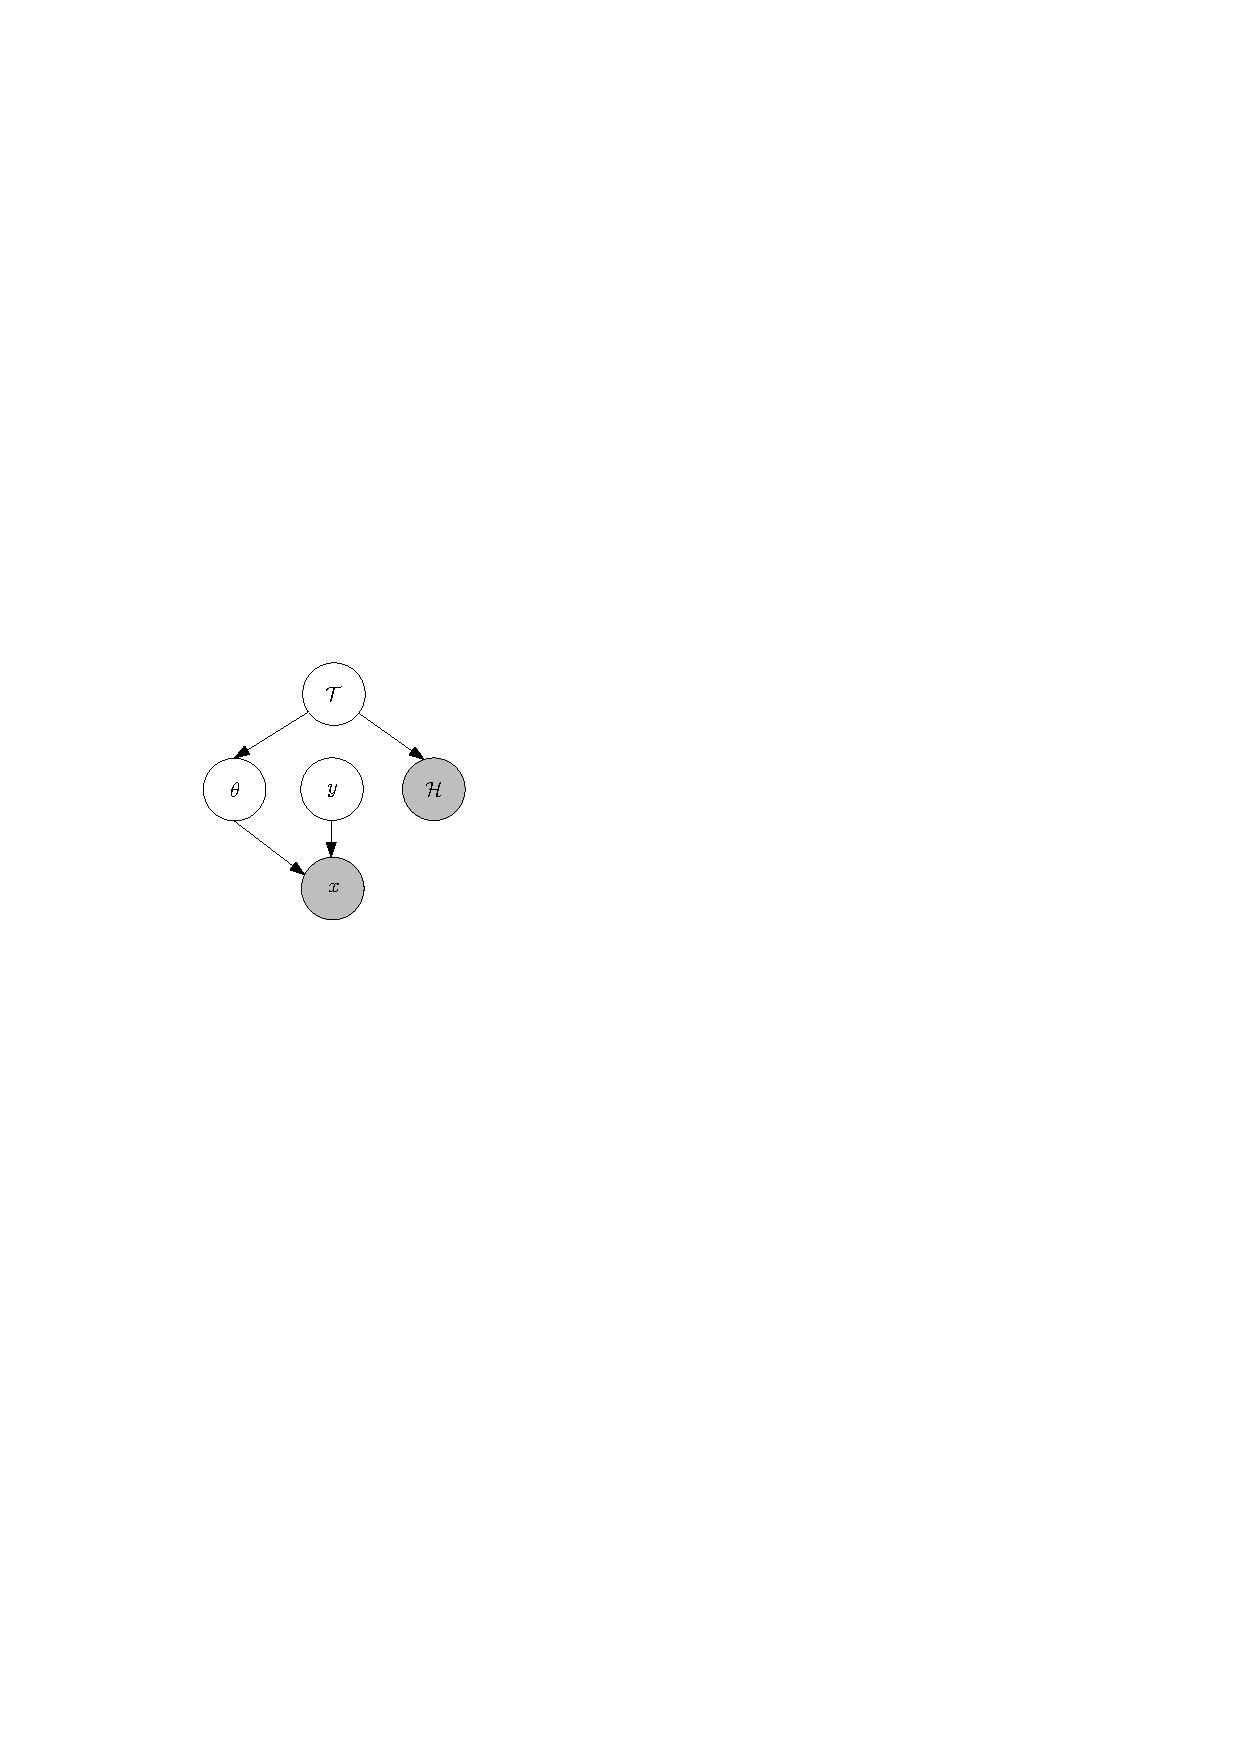
\includegraphics{generative.pdf}
  \caption{{\bf Relaxing the Closed World Assumption}}
  \label{generative}
\end{figure}

\begin{comment}
\subsection{Named Entity Classification \citep{Ritter11}}
To heuristically generate training data for named entity classification, we use large dictionaries of entities gathered
from Freebase.  In many cases, an entity will be ambiguous, taking different types in different contexts (e.g. the ``Amazon'' example above).

Each entity is modeled as a mixture of types, where the set of types associated with each entity is constrained based on the Freebase dictionaries.
The latent variables model the type of each individual entity mention in context.

This approach was shown to outperform the co-training approach of Collins and Singer, in addition to a supervised baseline in an evaluation
of named entity categorization on Twitter.

\subsection{Distantly Supervised Information Extraction}
Here we can take a very similar approach to that described for Named Entity Classification.  Each pair of entities can be modeled
as a mixture of relations, for example (\emph{Steve Jobs}, \emph{Apple}) would be modeled as a mixture of the relations 
\{{\sl ceoOf}, {\sl founder}, ...\}.

The latent variables model the relation mentioned in each sentence.

The work by \cite{Hoffmann11} is very relevant here, as they present a probabilistic graphical model for capturing
both aggregate and local extraction decisions.  Their approach is based on a discriminative model in contrast to the generative model
proposed here.

\subsection{Temporal Reference Resolution}
The idea here is to model temporal references using a constrained HMM.  Each sentence mentioning an event will be associated with a unique date
on which the event takes place.  The sequence of words in the sentence will be modeled using a constrained HMM, where the probability of transitioning
into a state not associated with the date of the event is set to 0.

Here the latent variables model whether each word is part of a temporal expression and what date properties they are associated with if so.

\section{Related Work}
\end{comment}


\bibliography{bib}
\end{document}
